\section{Domaine}

La réalité augmenté est un concept visant à enrichir la perception que nous avons avec le monde réel avec lequel nous interagissons. Cela se manifeste par un ensemble de technique informatique permettant d'incruster des éléments virtuelles de façon cohérente au sein d'élements réels (photographie, vidéo filmé ...), le tout en \gls{realtime}. 
Bien qu'on trouve souvent des cas lié à la perception visuelle, la \gls{ra} s'applique également à la perception sonore comme c'est le cas par exemple avec une application du CNAM pour les visites
de musées par les malvoyants, en produisant un effet sonore à proximité de l'oeuvre exposé (ref). Les applications de réalité aumgmenté sont diverses et variés et touche de plus en plus de domaine, tel que le jeux vidéo, la médécine, le tourisme, ou encore le commerce.

\begin{figure}[!ht]
\centering
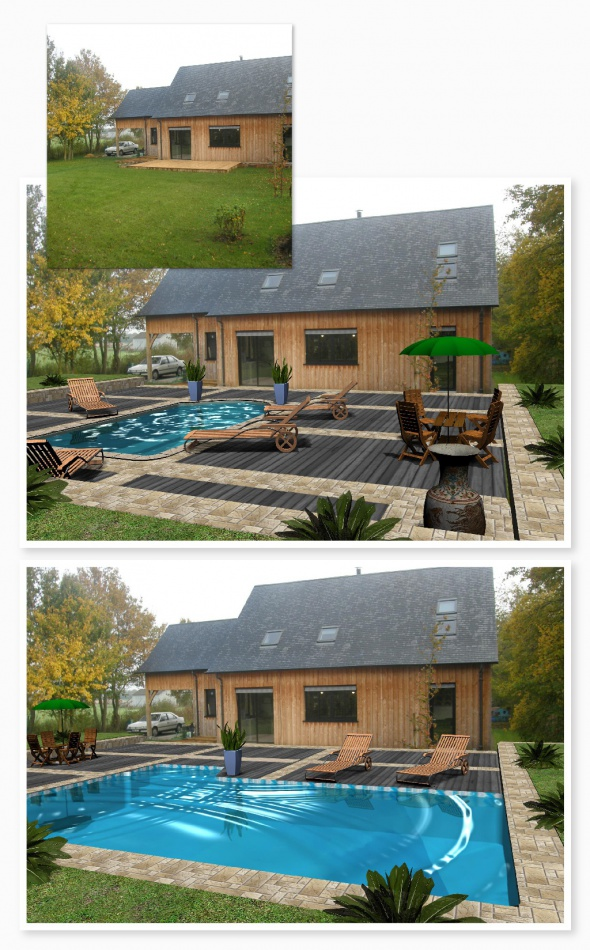
\includegraphics[width = 5.5cm] {images/exempleLC3DPool.jpg} 
\caption{Exemple de réalité augmentée avec \gls{lc3d} Pool de Logyline}
\label{fig:exempleRA}
\end{figure}

Une des notion importantes de la \gls{ra} est le fait de pouvoir assurer la cohérence entre la scène virtuelle (ensemble des element virtuelle) et la scène réelle.En ce qui concerne la suite de logiciel \gls{lc3d}, cela implique quatres contraintes principales :

\begin{itemize}
    \item Détection du sol: l'objet virtuel doit être automatiquement posé sur le sol
    \item Respect des mesures : cohérence entre la taille des objets virtuels avec celle des objets réel figurant sur l'image 
    \item Gestion des occlusions : si l'objet virtuel est positionné de façon à se trouver derrière un élément réél de la photo (mur, arbre, etc) alors le masquage de l'objet doit être visible
    \item Prise en compte des jeux de lumière (ombres, reflets) entre les différent objets.
\end{itemize}

C'est autour de cette notion que se déroulera mon stage, il convient alors de savoir comment cela est traité dans les logiciels de Logyline. 